
\begin{frame}{Strand- og havjagt}
    
    \begin{columns}[T]
        \begin{column}{0.58\textwidth}
            \begin{itemize}
                \item Pramjagt (passiv) - venter på trækkende fugle
                \item Motorbådsjagt (aktiv) - sejler med vinden mod fuglene
                \item Max hastighed 5 km/t under jagt
                \item Max hastighed 18 km/t før/efter jagt
                \item Gratis på fiskeriterritoriet
                \item Vær påpasselig med vejr, udstyr og sikkerhed
                \item Haglgevær anvendes
                \item Der anvendes typisk ikke hunde til jagtformen
            \end{itemize}
        \end{column}
        
        \begin{column}{0.4\textwidth}
            \centering
            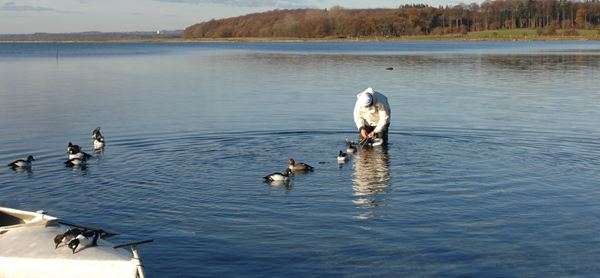
\includegraphics[width=\textwidth,height=0.85\textheight,keepaspectratio]
                {Billeder/Jagtformer/havjagt}
            % Alternativt brug en af disse stilrene billeder:
            % \includegraphics[width=\textwidth]{highseat-snow-forest-hunter.jpg}
            % \includegraphics[width=\textwidth]{hunter-leaning-tree-rifle.jpg}
        \end{column}
    \end{columns}
    
\end{frame}